\documentclass{article}
\usepackage[ttscale=0.825]{libertine}
\usepackage[libertine]{newtxmath}
\usepackage{amsmath,amstext,amssymb}
\usepackage{graphicx}
\usepackage{sectsty}
\usepackage{siunitx}
\usepackage{parskip}
\usepackage{booktabs}
\usepackage{hyperref}
\hypersetup{colorlinks=true,urlcolor=blue}

\newcommand{\oderiv}[2]{\ensuremath{\frac{\text{d}#1}{\text{d}#2}}}

\begin{document}
\allsectionsfont{\normalfont\sffamily\bfseries}
\begin{center}
    \large{CVEN 306 Laboratory Exercise}

    \Large{\textsf{\textbf{Thermal Conduction in a Composite}}}
\end{center}

\vspace{0.25truein}
\section*{Objectives and Learning Outcomes}
This laboratory exercise will reinforce the concepts you learned both on composite
materials and on thermal properties.  You will learn (1)~to compute the effective
\textit{heat transfer coefficient} of a composite wall, (2)~to determine the
\textit{steady-state} temperature profile through a composite, and (3)~to design
a composite wall with optimum heat transfer resistance for a given density.

\section*{Background}
\subsection*{Thermal Conductivity}
Recall that Fourier's Law for heat conduction
in one direction through a material is given by
\begin{equation}
    Q = -k A \oderiv{T}{x}
    \label{eq:Fourier}
\end{equation}
\begin{itemize}
    \item $Q$ = heat transfer rate (\si{\joule\per\sec} or \si{\watt}),
    \item $k$ = thermal conductivity (\si{\watt\per\meter\per\kelvin}),
    \item $A$ = cross-sectional area perpendicular to the heat flow direction (\si{\meter\squared}),
    \item $T$ = temperature (\si{\degreeCelsius} or \si{\kelvin}), and
    \item $x$ = distance in the heat flow direction (\si{\meter})
\end{itemize}

\subsection*{Steady State Conditions}
As we learned when studying diffusion, the special case of \textit{steady-state} heat transfer in 
a system means that the rate of transfer is equal everywhere in that system.
By examining Eq.~(\ref{eq:Fourier}), this means that $k\cdot$d$T$/d$x$ is the
same everywhere at steady state.  In particular, within any region where $k$ is
constant, d$T$/d$x$ is also a constant, and this means that $T$ versus $x$ is
a linear profile.  Furthermore, if $k$ is greater or less in some other region
of the system, then the slope of that linear temperature profile will decrease
or increase in magnitude, respectively, to keep the product $k\cdot$d$T$/d$x$ fixed.

To summarize, imagine a system where the thermal conductivity between position $x_1$ and $x_2$ is
$k_1$ and between position $x_2$ and $x_3$ is $k_2$. At steady state Eq.~(\ref{eq:Fourier})
means that
\begin{equation}
    \frac{Q}{A} = -k_1 \frac{T_2 - T_1}{x_2 - x_1} = -k_2 \frac{T_3 - T_2}{x_3 - x_2}
    \label{eq:steadystate01}
\end{equation}
This is illustrated for such a system in Figure~\ref{fig:twowall}.

\begin{figure}
    \centering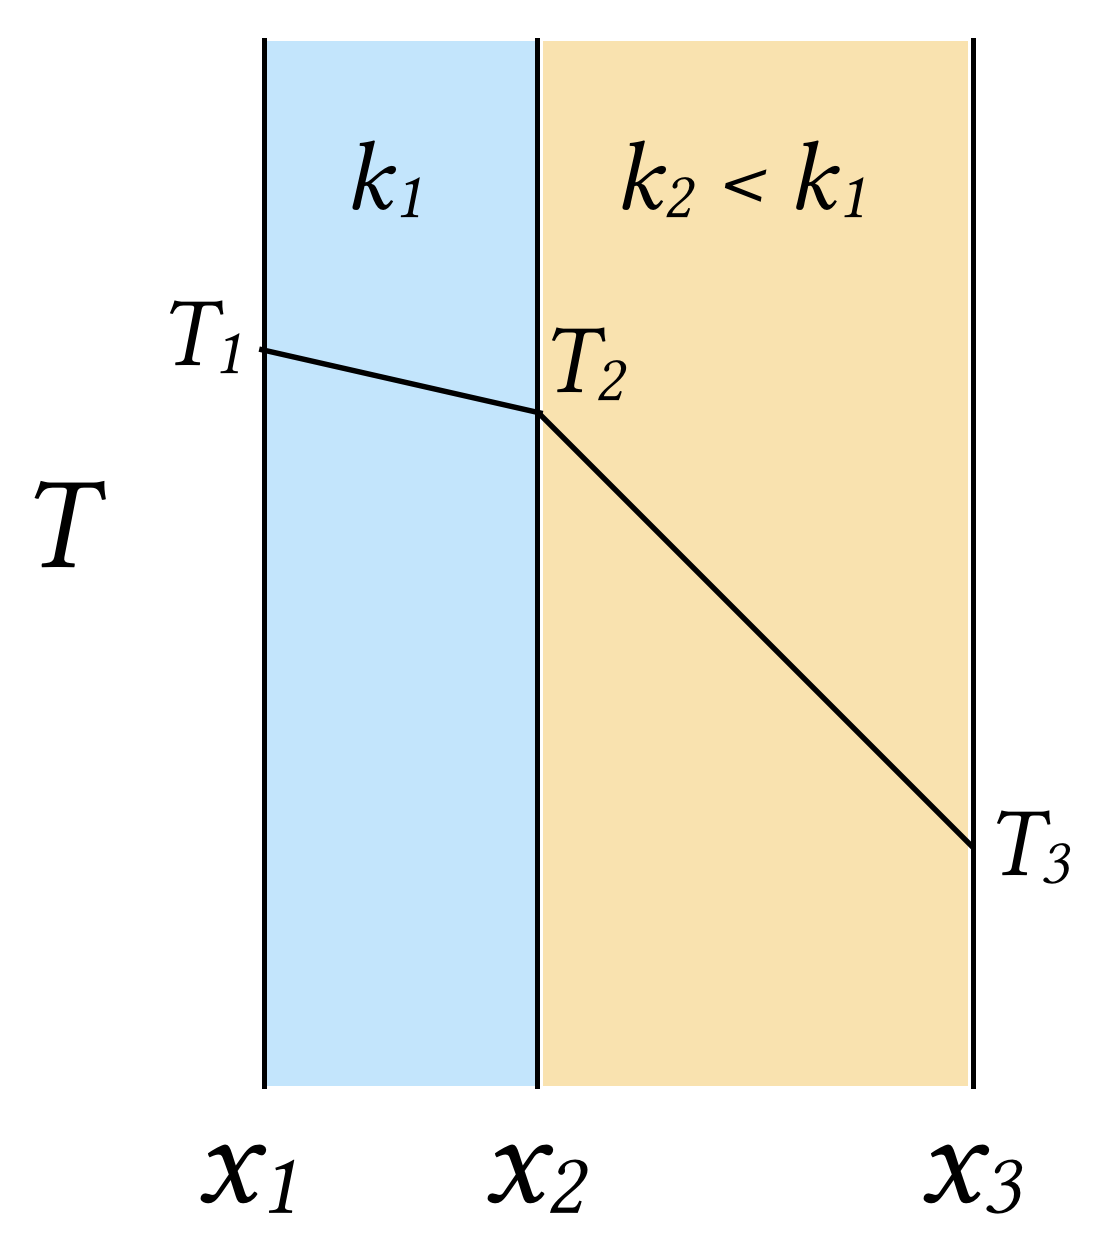
\includegraphics[scale=0.2]{Figure01.png}
    \caption{\label{fig:twowall} Steady-state temperature profile in a two-component wall.}
\end{figure}

\subsection*{Heat Transfer Coefficients}
Thermal \textit{conduction} refers to the transfer of thermal energy by atomic vibrations or by
the motion of free electrons.  In a flowing fluid, heat can also be transferred
from one point to another by \textit{convection} as the moving
fluid carries its thermal energy along with it.  In these cases, we make an
analogy to thermal conduction by defining a parameter called the
\textit{heat transfer coefficient}, $h$,
between two locations with temperatures $T_1$ and $T_2$, according to this relation:
\begin{equation}
    Q = -h A \left( T_2 - T_1 \right)
    \label{eq:hxfer}
\end{equation}
where $Q$ is still the rate of thermal energy transferred from position 1 to position 2 and $h$
has units of (\si{\watt\per\meter\squared\per\kelvin}).

\subsection*{1D Wall Composite}
You have learned that when the $n$ components of a composite material are arranged
\textit{in series}, the effective value of any transport property $k$ is given by
\begin{equation}
    \frac{V}{k_{\text{e}}} = \sum_{i=1}^n \frac{V_i}{k_i}
    \label{eq:Series1}
\end{equation}
where $V$ is the total composite volume, and $V_i$ and $k_i$ are the volume and transport property
of component $i$, respectively.  If the cross-sectional area, $A$, of the wall is constant then this
equation becomes
\begin{equation}
    \frac{L}{k_{\text{e}}} = \sum_{i=1}^n \frac{L_i}{k_i}
    \label{eq:Series2}
\end{equation}
where $L$ is the total thickness of the wall and $L_i$ is the thickness of layer $i$.

Imagine a composite wall between two fluids that can transfer heat by convection to or
from the wall surfaces, as shown in Figure~\ref{fig:twowallfluids}, and assume that the
temperatures of the fluids far away from the walls are constant at $T_L$ on the left
and $T_R$ on the right.
The whole system can be treated as a series composite to define the
\textit{effective heat transfer coefficient}, $U$, by just adding the two terms for the
fluids to Eq.~(\ref{eq:Series1}),
\begin{equation}
    \frac{1}{U_{\text{e}}} = \frac{1}{h_L} + \sum_{i=1}^n \frac{L_i}{k_i} + \frac{1}{h_R}
    \label{eq:Series3}
\end{equation}

\begin{figure}
    \centering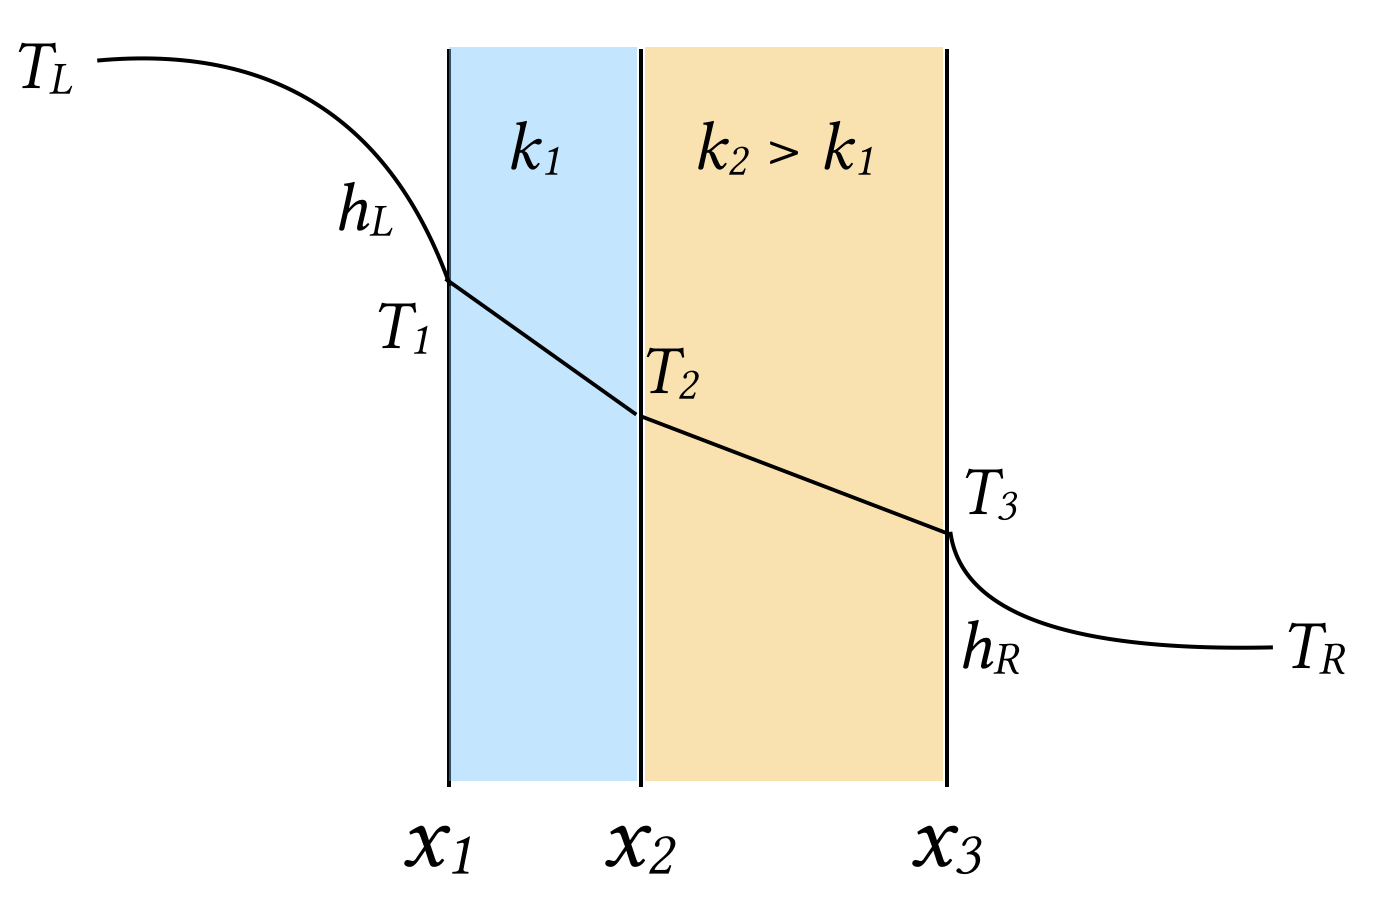
\includegraphics[scale=0.3]{Figure02.png}
    \caption{\label{fig:twowallfluids} Steady-state temperature profile in a
        two-component wall between two fluids.}
\end{figure}

\section*{Lab Tasks}
\subsection*{Task 1}
Derive Eq.~(\ref{eq:Series2}) from Eq.~(\ref{eq:Series1}) when the wall cross-sectional
area is constant.

\subsection*{Task 2}
For the remaining tasks you will be working with three-layer composite walls made of two or
more of the materials given in Table~\ref{tab:mats}.

\begin{table}
    \caption{\label{tab:mats} Material properties for lab exercise.}
    \begin{center}
    \begin{tabular}{lSS} \toprule
        \textbf{Material} & \multicolumn{1}{c}{Density} & \multicolumn{1}{c}{Thermal Conductivity} \\
        & \multicolumn{1}{c}{(\si{\gram\per\centi\meter\cubed})}
    & \multicolumn{1}{c}{(\si{\watt\per\meter\per\kelvin})} \\ \midrule
    Polypropylene & 0.9 & 0.15 \\
    Stainless Steel & 7.8 & 20.0 \\
    Aluminum & 2.7 & 220.0 \\ \bottomrule
\end{tabular}
\end{center}
\end{table}

Open a web browser and navigate to the Engineering ToolBox website:
\begin{center}
    \url{https://www.engineeringtoolbox.com/overall-heat-transfer-coefficient-d_434.html}
\end{center}

About halfway down the page you will see a calculator right below a figure similar to
Figure~\ref{fig:twowallfluids}.  You will use this calculator to complete some parts of this
exercise [\textbf{Note}: the calculator uses different symbols for some of the parameters
than what were used in class or in this lab sheet.]

Experiment with the calculator using any two of the three materials in Table~\ref{tab:mats}.
After getting some practice, answer the following questions and support
the answers by analyzing Eq.~(\ref{eq:Series3}):
\begin{enumerate}
    \item How does the effective heat transfer coefficient depend on the area, $A$?
    \item How does the heat transfer rate depend on the area?
    \item If the thickness of each layer is the same, does the ordering of the
        layers influence the effective heat transfer coefficient?  What about the
        heat transfer rate?
    \item How do the effective heat transfer coefficient and the heat transfer
        rate change with the difference in temperatures of the two fluids?
\end{enumerate}

\subsection*{Task 3}
A three-layer wall is constructed with the outside layer (left) being \SI{0.1}{\meter} of
stainless steel, the middle layer being \SI{0.3}{\meter} of polypropylene, and the
inside layer being \SI{0.2}{\meter} of aluminum.  Let the outside temperature far from
the wall be \SI{200}{\degreeCelsius}, and let the inside temperature far from the wall
be \SI{25}{\degreeCelsius}. The heat transfer coefficient at both walls is
\SI{0.2}{\watt\per\meter\squared\per\kelvin}.
\begin{enumerate}
    \item Calculate the steady-state temperature profile between the outer wall surface and
the inner wall surface using Eqs.~(\ref{eq:steadystate01}) and~(\ref{eq:hxfer}).
    \item Plot the steady-state temperature profile between the outside surface and the inside
surface.
    \item What are the steady-state temperatures at the outer wall surface and the inner
        wall surface?
\end{enumerate}

\subsection*{Task 4}
Design a three-layer composite wall with the \textit{minimum possible} effective heat transfer coefficient
subject to the following engineering constraints:
\begin{itemize}
    \item You must choose materials from among the three given in Table~\ref{tab:mats}.
    \item $h_L = h_R = \SI{5}{\watt\per\meter\squared\per\kelvin}$.
    \item The wall must be \SI{1}{\meter} thick.
    \item The overall density of the wall must be between
        \SI{2.0}{\gram\per\centi\meter\cubed} and
        \SI{4.0}{\gram\per\centi\meter\cubed}.
\end{itemize}
Describe the optimized wall design and determine its effective heat transfer coefficient.
[\textbf{Hint}: If you don't know or can't decide how to solve this problem, I recommend
using the method of \textit{graphical linear programming}. There is a section attached to
the end of
this document explaining what this method is and how to use it for optimization.  If you
have never used it before, I think you will find that it is nice technique to add to your
skill set.]

\section*{Reporting}
Complete all the tasks, explaining your answers fully to all the questions.  Show all the calculations
you made for Tasks 3 and 4 in a neat and logical sequence. Your plot in Task 3 must be neatly and fully
labeled.  Assemble all your work in a single PDF document, with each task clearly delineated.
Make sure that your name and UIN are clearly shown on the first page.

Submit your completed PDF document on eCampus no later than 2 April 2020.
% (\href{mailto:gogaltha31@email.tamu.edu}{gogaltha31@email.tamu.edu}).

\newpage
\section*{Graphical Linear Programming}
The most important thing to understand at the beginning is that linear programming is \textsc{not}
computer programming or anything like that.  You can easily perform the method described here with
a pencil, paper, and calculator.

Linear programming is one of the simplest ways to perform optimization on fairly complex systems
that have multiple constraints.  These kinds of problems arise all the time in engineering
practice, so it is extremely useful to have a way to solve them.

\textbf{Example}: Suppose you work in a factory that makes two
particular gadgets, a Fuzzy and a Buzzy.  Each Fuzzy sells for \$5, and it is made by
connecting three Gizmos to twelve Fizmos.  Each Buzzy sells for \$7, and it is made by
connecting two Gizmos to two Fizmos.  The factory has 240 Gizmos and 100 Fizmos. 
Assuming that the factory sells every gadget they produce, how many Fuzzys and Buzzys
should the factory produce to maximize their revenue?

All optimization problems like this involve something that is to be maximized or minimized,
in this case the factory's revenue, as well as one or more \textit{constraints}, in this
case the number of parts needed to make each product and the total number of each part
that is available.  Linear programming enables one to solve these kinds of problems by
representing the constraints as \textit{linear inequalities}, and then graphing all the
inequalities to identify the space of possible solutions.  The optimum solution must 
lie within this space to satisfy the constraints, and linear programming provides
a mechanism to identify that solution.

Of course there is an entire mathematical theory of linear programming which provides
proofs of the methods we are about to use.  Those of you who are interested can find
this deeper theory online.
However, we will just work through the example problem above step-by-step to illustrate
the process.  You can then apply the same process to Task~4 in the lab exercise.

\subsubsection*{Step 1: Write the objective function}
The \textit{objective function} is a mathematical description of the quantity that must
be optimized.  In this case, it is the total revenue for the factory.  We will let
$F$ be the number of Fuzzys and $B$ be the number of Buzzys.  Then the revenue (total
amount of money made by selling all the Fuzzys and Buzzys) is given by
\begin{equation}
    R = 5 F + 7 B
    \label{eq:objectivefn}
\end{equation}
in which the coefficients are the selling price of the respective gadget.

\subsubsection*{Step 2: Write the constraints as linear inequalities}
This part is sometimes a little trickier to figure out because each constraint must
be expressed as an inequality.
Here is a list of the contraints that we see from the problem, written in words:
\begin{enumerate}
     \item Each Fuzzy requires three Gizmos and each Buzzy requires two
         Gizmos, but there are only 120 Gizmos available.  We can write this
         mathematically as $3F + 12 B \le 240$, or $F \le 80 - 4B$
     \item Each Fuzzy requires two Fizmos and each Buzzy requires two
         Fizmos, but there are only 150 Fizmos available.  We can write this
         mathematically as $2F + 2B \le 50$, or $F \le 50 - B$.
      \item The total number of Fuzzys made cannot be negative, so $F \ge 0$.
         The same holds for the Buzzys, so $B \ge 0$.
\end{enumerate}
In summary, we have four inequalities:
\begin{align}
F &\le 80 - 4 B \\
F &\le 50 - B \\ 
F &\ge 0 \\
B &\ge 0 
\end{align}

\subsubsection*{Step 3: Plot all the inequalities on the same graph}
Make a graph in which the $y$-axis is the number of Fuzzys and the $x$-axis
is the number of Buzzys.  Then plot each inequality as a line and shade the
region above or below the line depending on whether the inequality is
$\ge$ or $\le$, respectively.  The figure shows such a plot, with the
green-shaded region satisfying all the inequalities.  This region is
called the \textit{feasible region}.

\begin{center}
    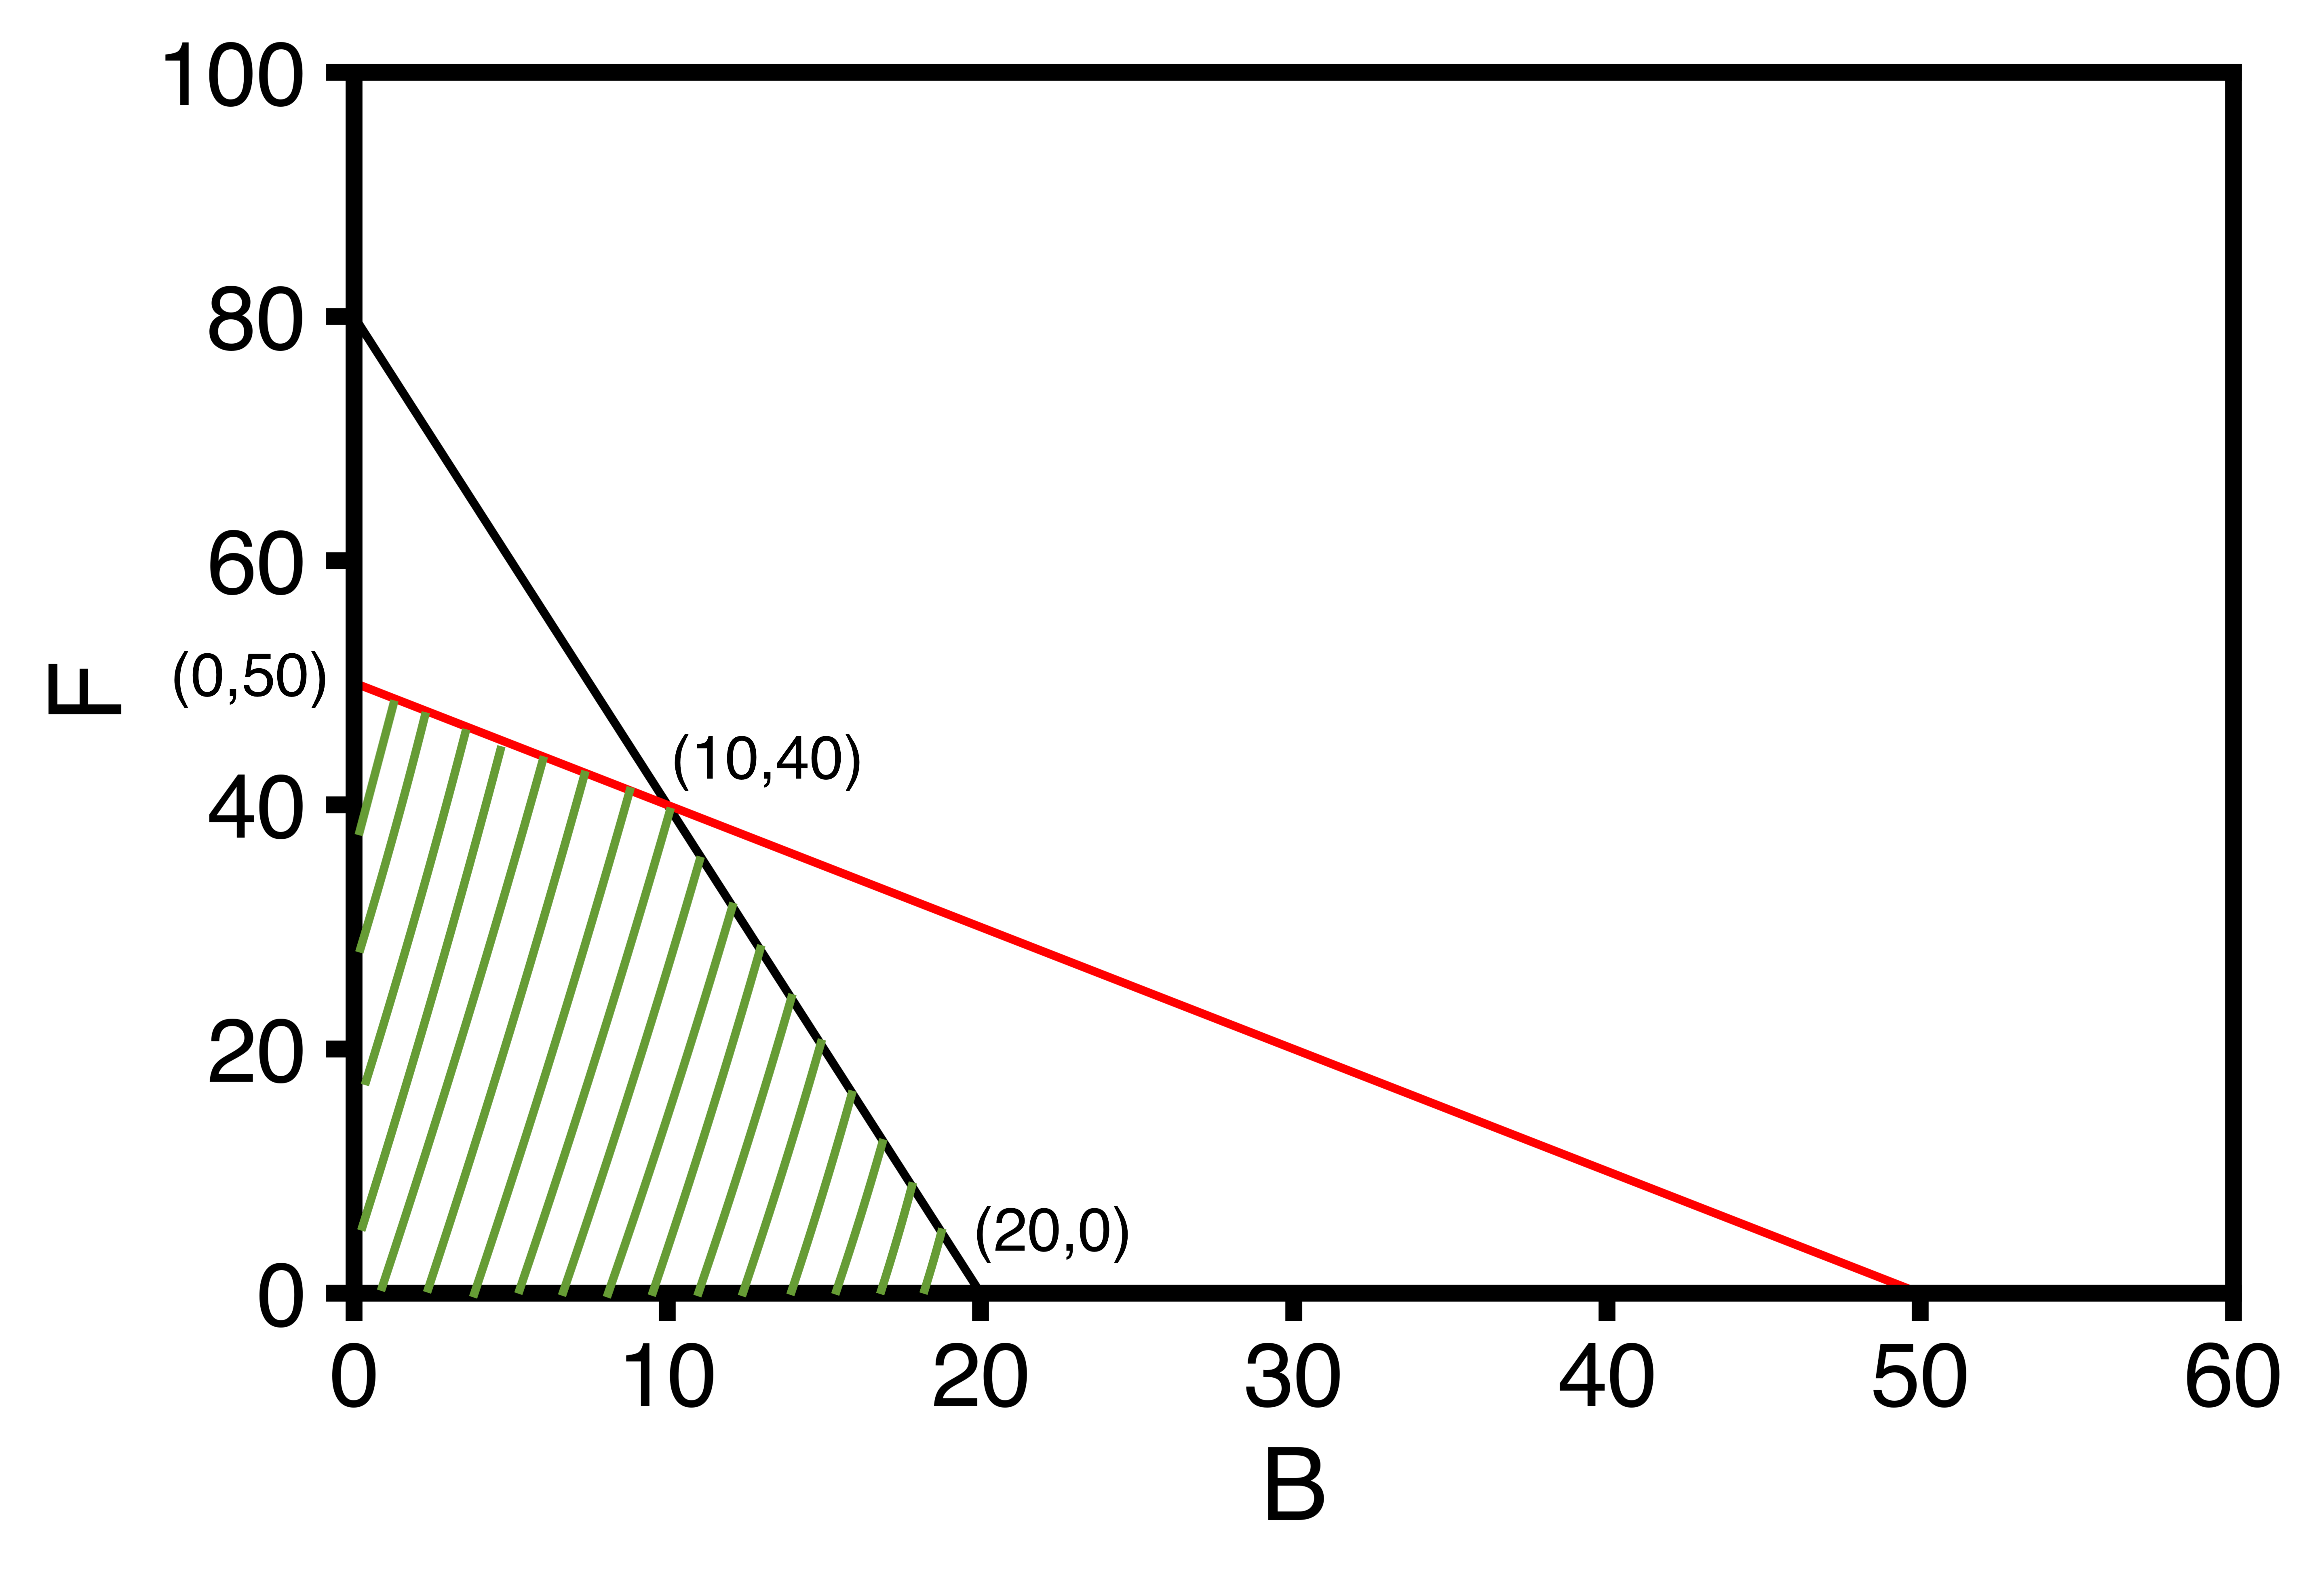
\includegraphics[scale=0.6]{FuzzyBuzzy.png}
\end{center}

\subsubsection*{Step 3: Test the vertices}
Without proving any of the following propositions, we will nevertheless use them:
\begin{itemize}
    \item \textbf{Proposition 1}: The feasible region is always either a convex polygon
        or an unbounded region of space.
    \item \textbf{Proposition 2}: If the feasible region is a convex polygon, then the
        objective function always has its maximum on one of the vertices (corners) of
        the feasible regions, and it also always has its minimum on another one of the
        vertices.
\end{itemize}
This means that all we need to do is use the $(B,F)$ values at each vertex of the feasible
region and calculate the objective function:

\begin{center}
\begin{tabular}{lll} \toprule
Vertex $(B,F)$ & Value of $R = 5 F + 7 B$ & Diagnosis \\ \midrule
$(0,0)$ & $0$ & Minimum \\
$(20,0)$ & $140$ & \\
$(0,50)$ & $250$ & \\
$(10,40)$ & $270$ & Maximum \\ \bottomrule
\end{tabular}
\end{center}

Therefore, the maximum possible revenue is \$270, and it happens when the factory
produces 40 Fuzzys and 10 Buzzys.

\subsubsection*{Application to Task 4}
That was an especially easy example.  Task 4 is more complicated but the
solution approach is exactly the same.  You may find it challenging to determine
all the different constraints to the problem, so here are a few additional pointers
for that task:
\begin{itemize}
    \item The objective function is the heat transfer coefficient, $U$, which needs to
        be minimized, but this means that $1/U$ needs to be maximized.
    \item The minimum and maximum allowed densities represent two constraints.
    \item The wall has a fixed thickness, so only two of the layer thicknesses
        are variable; the third layer thickness is determined by the other two.
        This imposes one constraint.
    \item No layer can have a negative thickness.  This imposes two constraints.
    \item In the previous tasks, did you observe that the ordering of the layer
        materials mattered for determining the heat transfer coefficient?
\end{itemize}
\end{document}
